\chapter{Event selection}
\label{evt_sel}
\section{Introduction}
\label{evt_sel_intro}
This chapter describes in detail the event selection criteria for the analyses, and how they were chosen. It starts by introducing the backgrounds that each of selection criterion is trying to reduce in order to get a higher ratio of number of signal events to background events, leading to a better sensitivity for the search. This is followed by the procedure for arriving at the best possible set of cuts. Both analyses were performed blinded~\cite{blind_analysis} in the signal region. All selection criterion and methods described below were developed without the knowledge of the observed data in the range of variable spectra where the signal is expected to be present. This is considered an optimal way of eliminating the unintended biasing of a result in a particular direction and is a standard methodology in particle physics analyses.  

\section{H125 analysis signature and backgrounds}
\label{h125_evt_selec}
The signature of the \hmue analysis final state consists of a muon that comes promptly from the Higgs and has a hard \pt spectrum, along with a softer electron that comes from the tau lepton, and missing transverse momentum from the tau decay. It is interesting to note that the signature is similar to the $\text{h} \to \Pgt_{\Pgm}\Pgt_{\Pe}$ decay that is allowed by the SM and since been observed, but with significant kinematic differences. In \hmue decay the $\Pgm$ comes directly from the Higgs resulting in its $\pt$ spectrum peaking and spreading out to much higher values. Also there are fewer neutrinos in \hmue, coming from the decay of the single $\Pgt$. The decay products of this highly boosted tau are closely aligned, leading to a narrow separation between the $\Pe$ and the \ptvecmiss in the azimuthal plane. The same is not true in the $\text{h} \to \Pgt_{\Pgm}\Pgt_{\Pe}$ decays. These differences are illustrated pictorially in Fig.~\ref{fig:htt_v_lfv}.






\begin{figure*}
\begin{center}
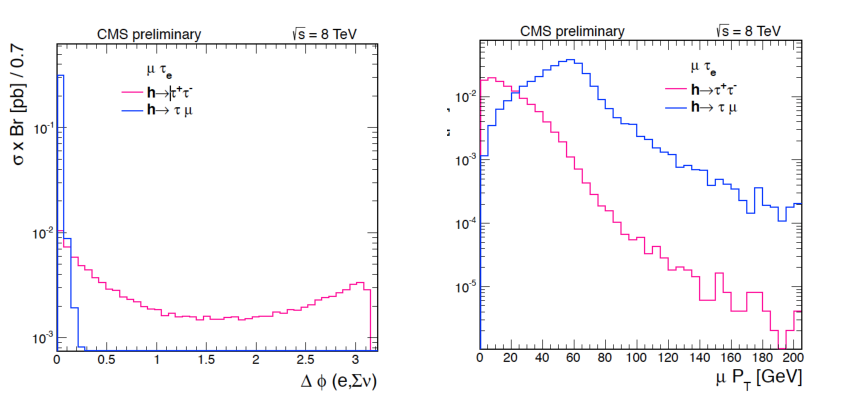
\includegraphics[width=0.8\textwidth,keepaspectratio]{plots_and_figures/chapter5/htt_v_lfv.pdf}
\caption{Illustration of the differences in $\Pgm_{\pt}$ and $\dphiemet$ spectrums in $\hmue$ and $\text{h} \to \Pgt_{\Pgm}\Pgt_{\Pe}$ processes.}
\label{fig:htt_v_lfv}
\end{center}
\end{figure*}

The most dominant backgrounds consists of \ztt events coming from Drell-Yan production and \ttb production. In \ztt events, one $\Pgt$ can decay to an $\Pe$ and the other to a $\Pgm$. This background peaks at lower values of $M_{col}$ than the signal events but there is significant overlap with the signal spectrum. In \ttb production, each of the top quarks can decay into a bottom and a $\PW$ with the $\PW$ bosons then decaying to a $\Pe$ and $\Pgm$. The other backgrounds are smaller and include (in no particular order) electroweak diboson production ($\PW\PW$, $\PW\PZ$ and $\PZ\PZ$), Higgs boson decays allowed by the SM ($\PH \to \Pgt\Pgt,\PW\PW$), $\PW\gamma^{(*)}+\text{jets}$ ,single top production, \wjets events, $Z\to\ell\ell$ $(\ell = \Pe, \Pgm)+\text{jets}$ and QCD multijet backgrounds. These backgrounds are described in more detail, along with there estimation and validation techniques in section~\ref{bg_val}.        


\subsection{Baseline selection and categorization}
\label{h125_evt_sel_bkg}
A baseline selection is defined first in order to ensure that we have clean and well-defined events faithful to the final state signature of the signal process. A tightly isolated and identified $\Pgm$ is thus required to be present along with an tightly identified and isloated $\Pe$ of opposite sign charge. They are required to be separated by $\Delta R > 0.3$. The tight identification criterion applied for $\Pgm$ and $\Pe$ have been described in sections~\ref{mu_recon} and~\ref{e_recon}. Isolation criterion, as measured by $I_\text{rel}$ (described in ~\ref{tau_recon}), are required to have values $I_\text{rel}^{\Pe} < 0.15$ and $I_\text{rel}^{\Pgm} < 0.1$. The $\pt$ of these candidates are required to be above minimal thresholds required by trigger, identification and isolation requirement. Both candidates are also required to be within the fiducial region of the detector. The $\Pgm$ is required to have $\pt^{\Pgm} > 26$\GeV and $|\eta^{\Pgm}|<2.4$.The $\Pe$ is required to have $\pt^{\Pgm} > 26$\GeV and $|\eta^{\Pgm}|<2.3$. Events with at least one jet arising from a b-quark (b-tagged jets) are also vetoed. Cleaning events with b-tagged jets reduce some contribution backgrounds which give rise to b-quarks such has \ttb and single top. As described in~\ref{jet_recon}, any event with one or more jets having $\pt>30$\GeV and within $\Delta R < 0.3$ of either lepton candidate is also rejected. Further, an event is rejected if it has additional $\Pgm$ or $\Pe$, or $\Pgt_{had}$ candidates. All the above baseline selection requirements have been summarized in Table~\ref{tab:h125_base_sel}  .In addition, all the events were required to pass isolated muon triggers with a $\pt$ threshold of 24 \GeV. The trigger selection has been described in detail in section~\ref{trigger}. The distributions of the \mcol and several other  kinematic variables are shown in Fig.~\ref{fig:h125_presel}  


\begin{table}[htpb]
 \begin{center}
 \caption{Baseline selection criteria for \hmue analysis.}
  \begin{tabular}{c|c|c} \hline
    Variable    &  $\Pgm$  & $\Pe$ \\ \hline
    $\pt $       & $>30$\GeV &  $>10$\GeV                                           \\
    $|\eta| $       & $<2.4 $ &  $<2.3$                                           \\
    $I_{\text{rel}}$  & $<0.15$ &  $<0.1$                                           \\
    \multicolumn{3}{c}{Cleaning requirements} \\\hline
    \multicolumn{3}{c}{ $\Delta R(\Pgm,\Pe) > 0.3$} \\
    \multicolumn{3}{c}{No additional $\Pgm$, $\Pe$ or $\Pgt_{had}$} \\
    \multicolumn{3}{c}{No b-tagged jets with $\pt>30$\GeV} \\
    \multicolumn{3}{c}{No jets with $\Delta R(\Pgm,jet)<0.4$ and $\pt>30$\GeV} \\
    \multicolumn{3}{c}{No jets with $\Delta R(\Pe,jet)<0.4$ and $\pt>30$\GeV }\\
    \hline
  \end{tabular}
  \label{tab:h125_base_sel}
  \end{center}
\end{table}


\begin{figure*}[!htpb]\centering
 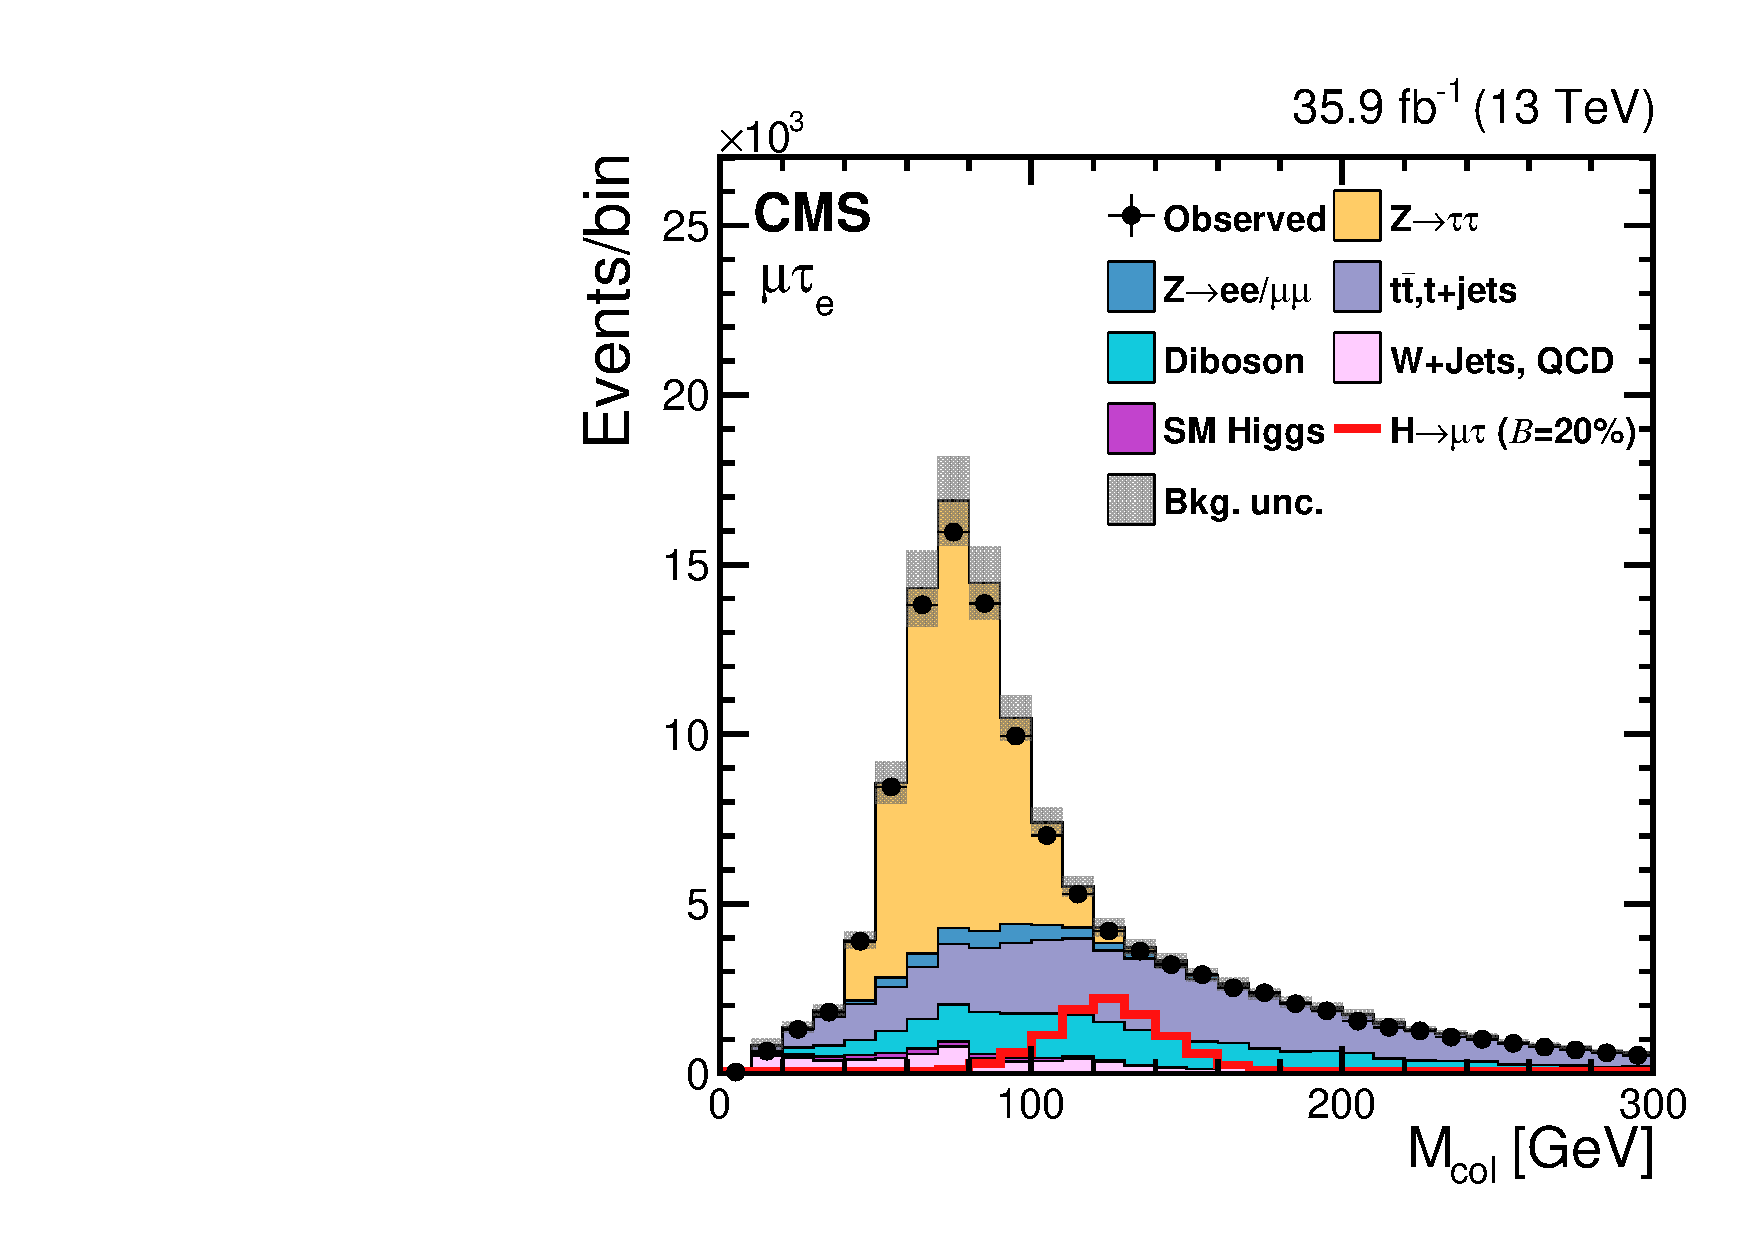
\includegraphics[width=0.315\textwidth]{plots_and_figures/chapter5/preselection/Figure_002-a.pdf}
 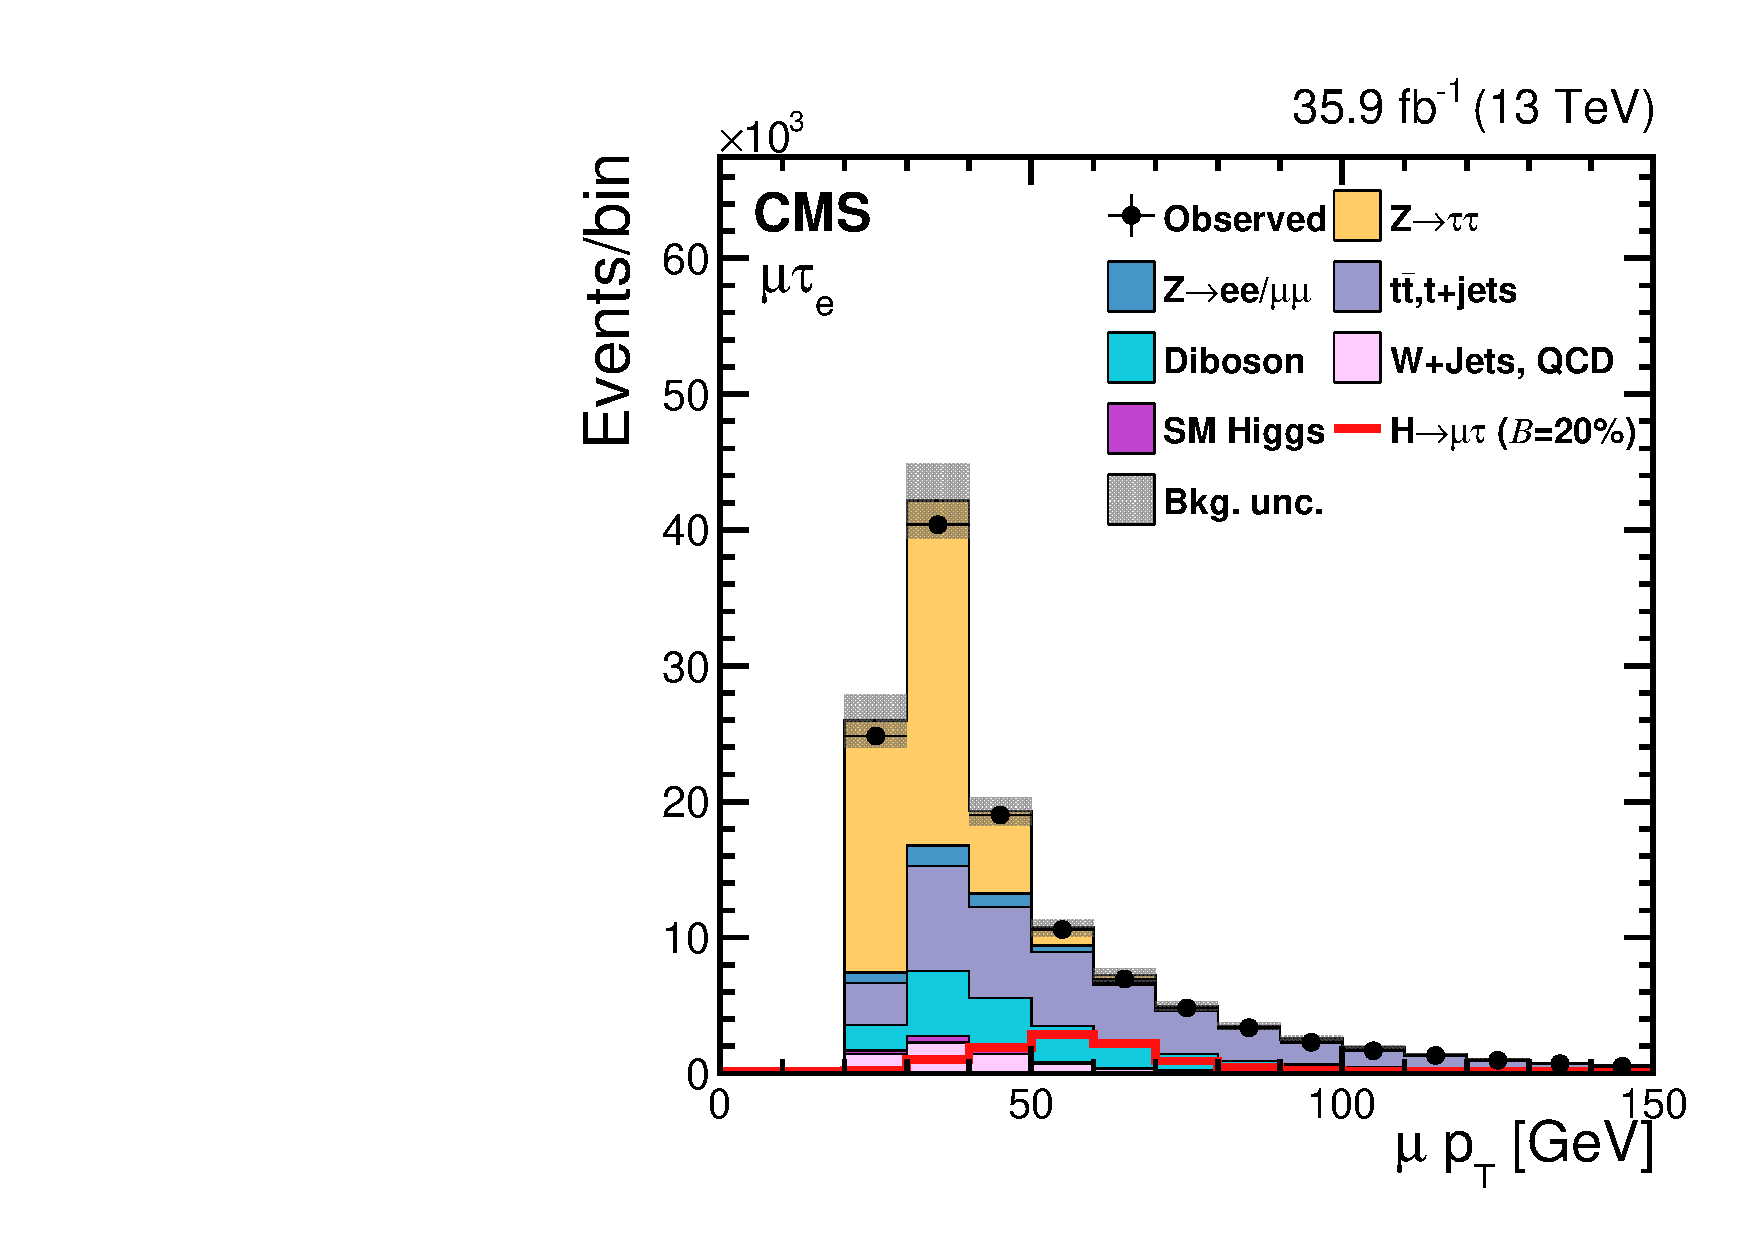
\includegraphics[width=0.315\textwidth]{plots_and_figures/chapter5/preselection/Figure_002-b.pdf} \\
 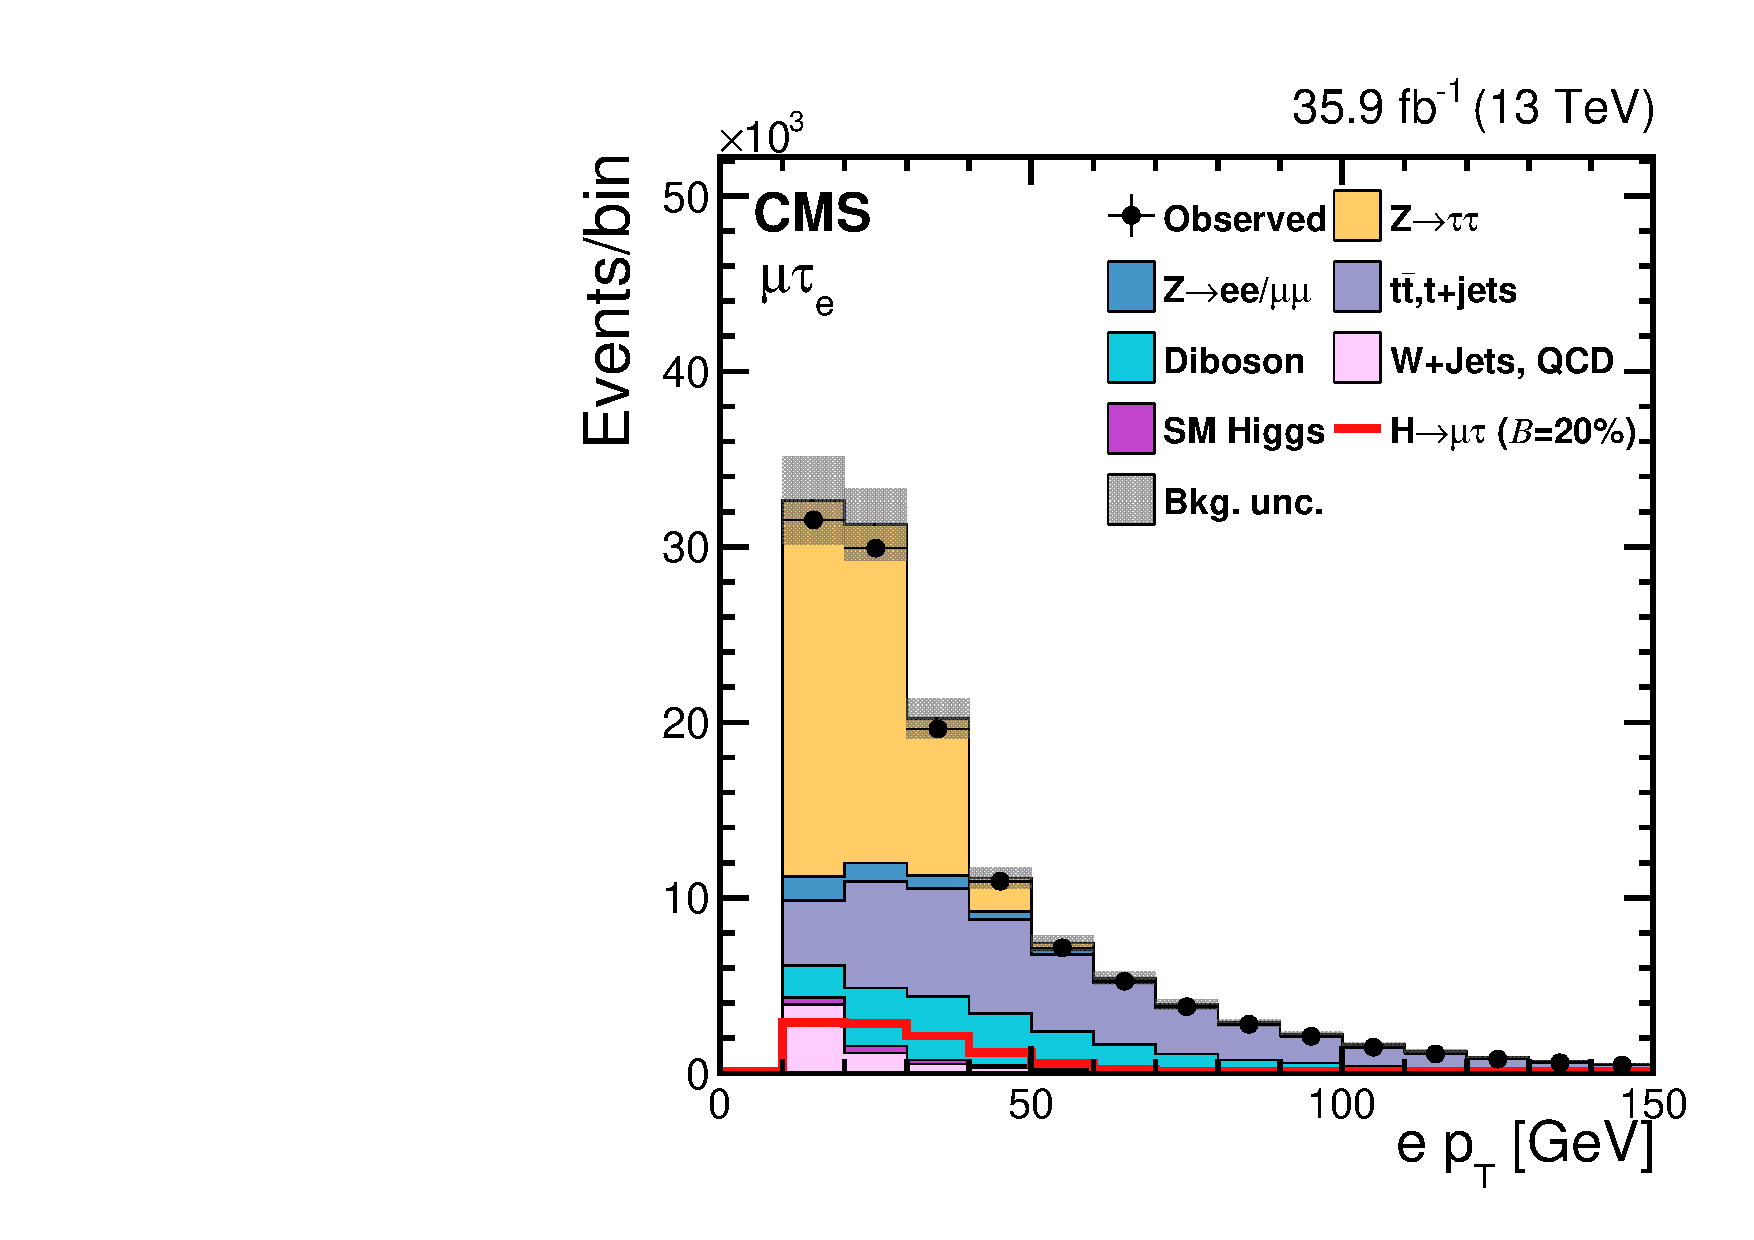
\includegraphics[width=0.315\textwidth]{plots_and_figures/chapter5/preselection/Figure_002-c.pdf}
 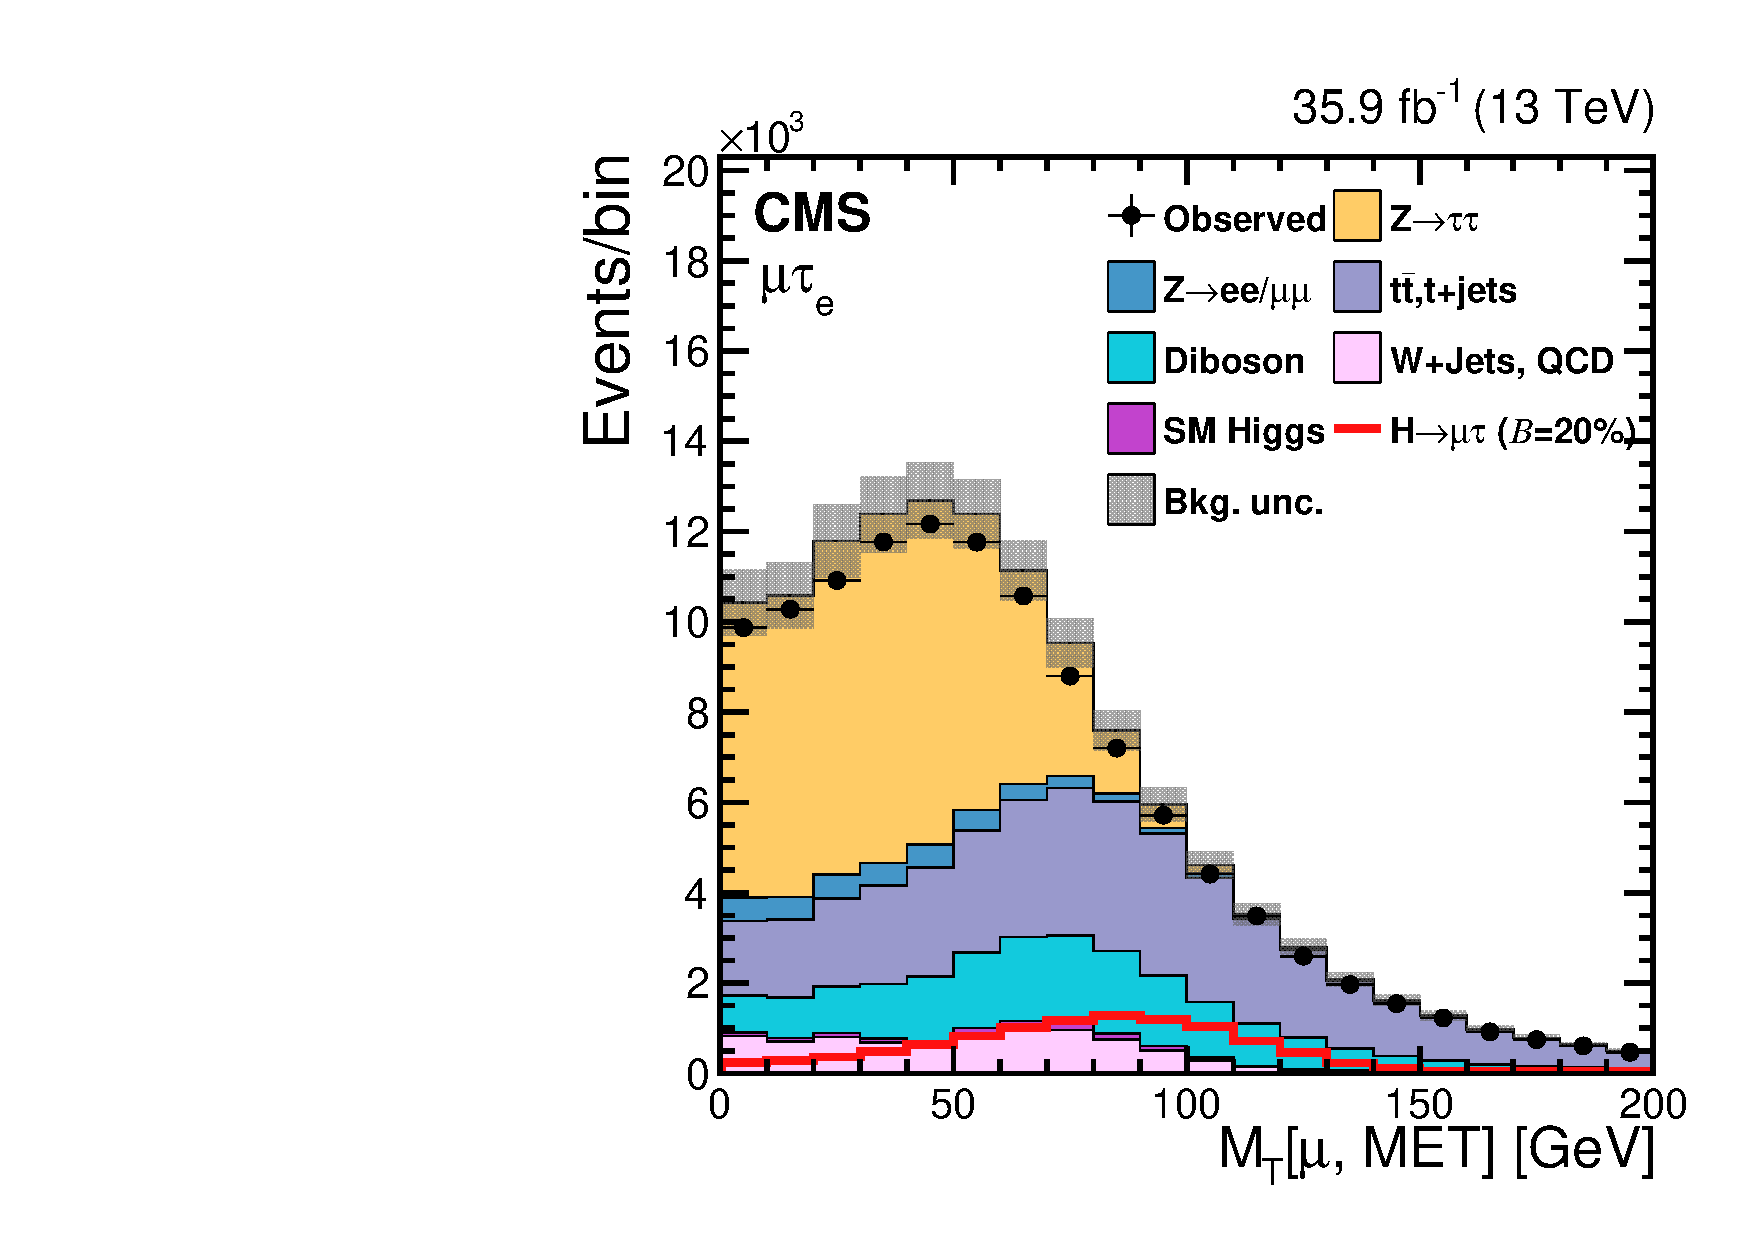
\includegraphics[width=0.315\textwidth]{plots_and_figures/chapter5/preselection/Figure_002-d.pdf}  \\
 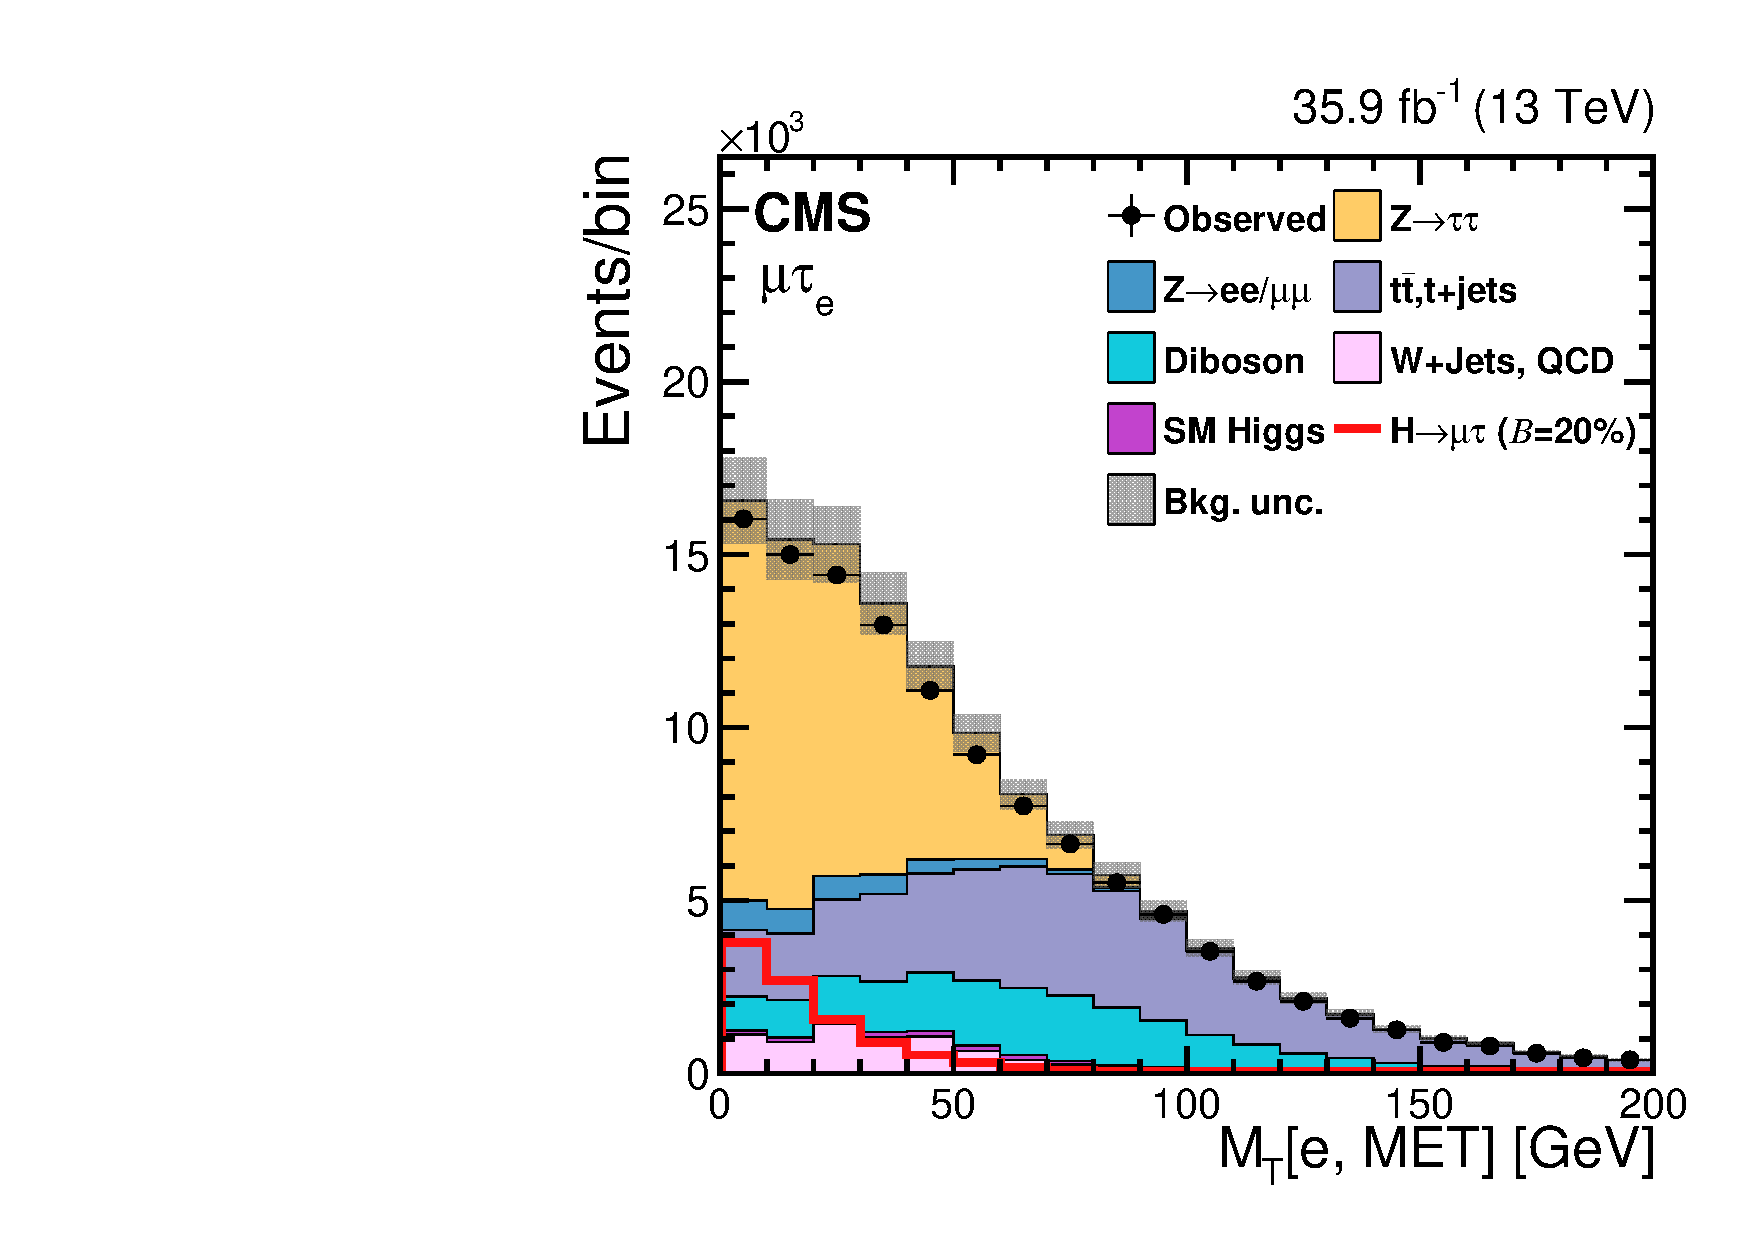
\includegraphics[width=0.315\textwidth]{plots_and_figures/chapter5/preselection/Figure_002-e.pdf}
 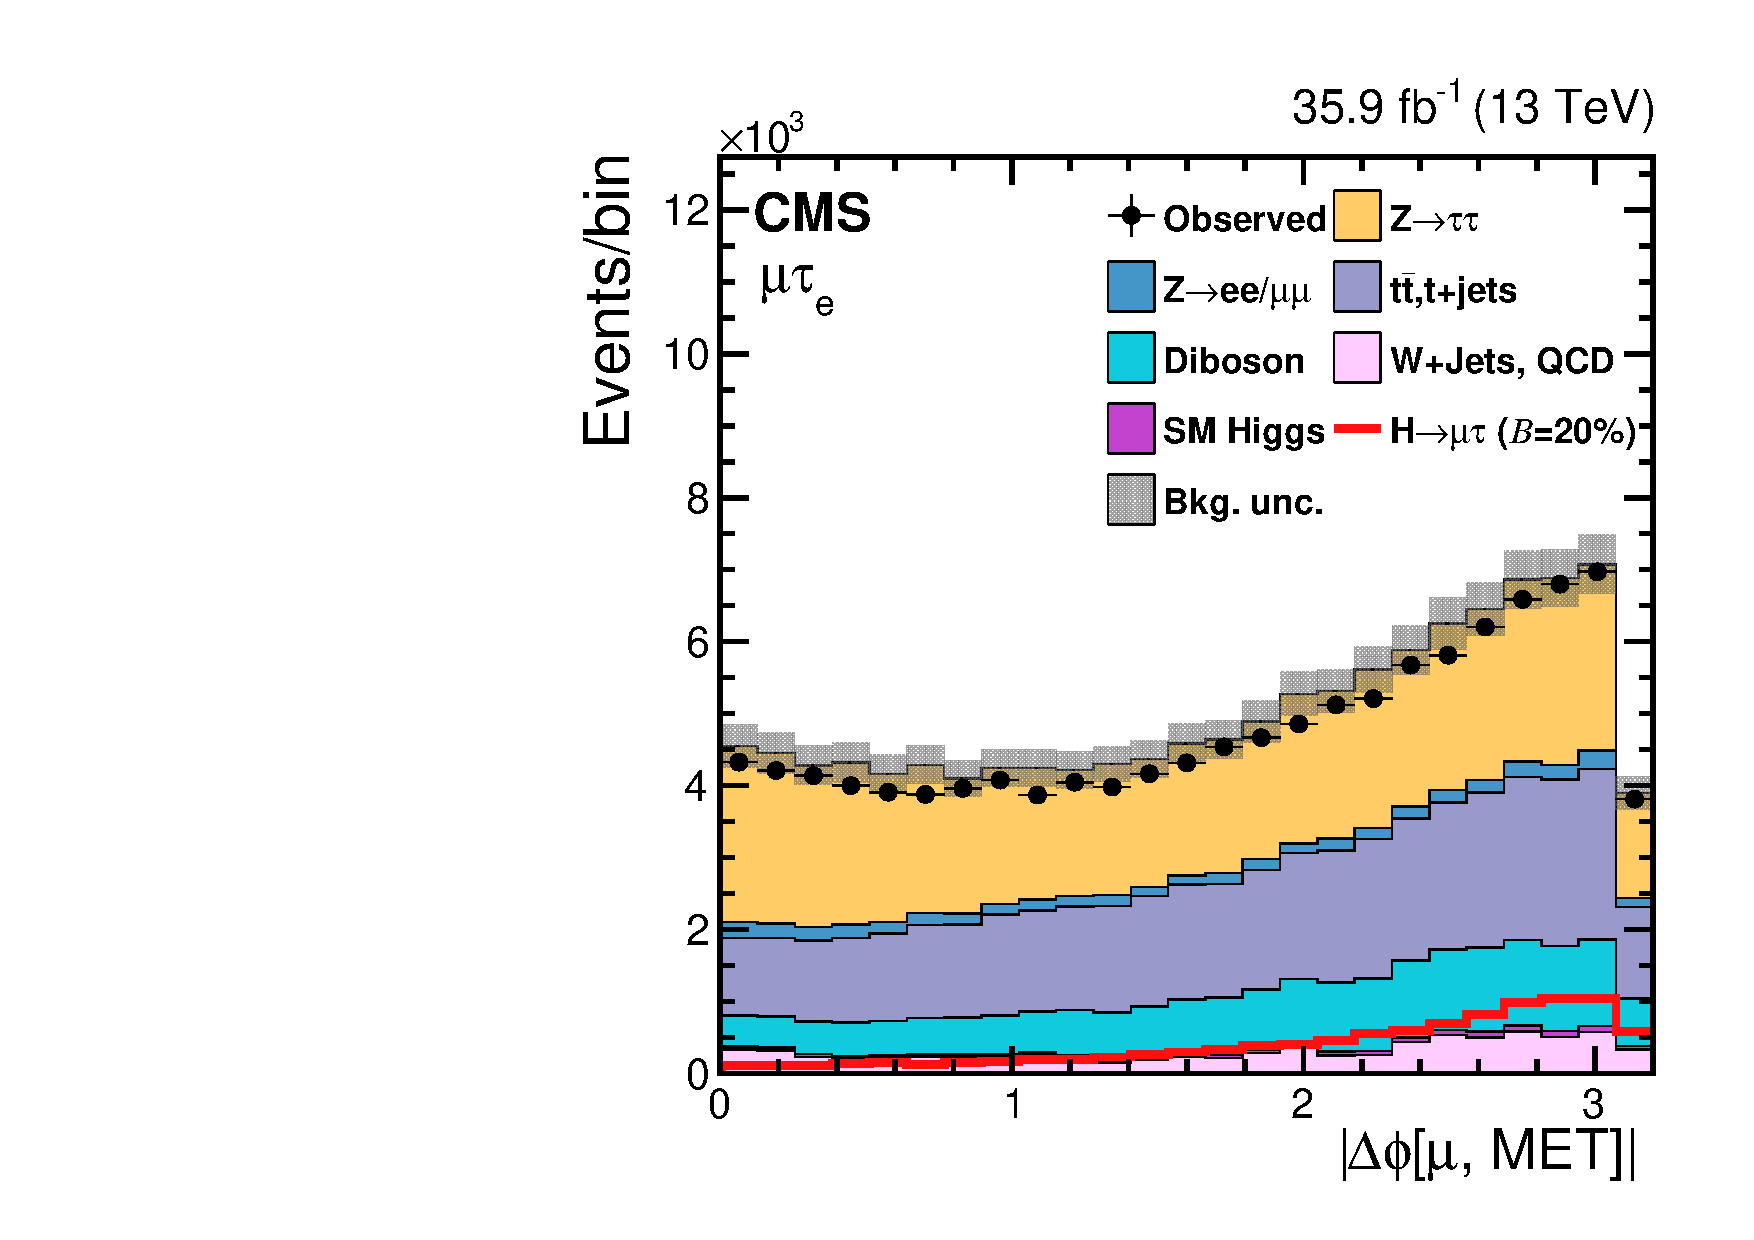
\includegraphics[width=0.315\textwidth]{plots_and_figures/chapter5/preselection/Figure_002-f.pdf} \\
 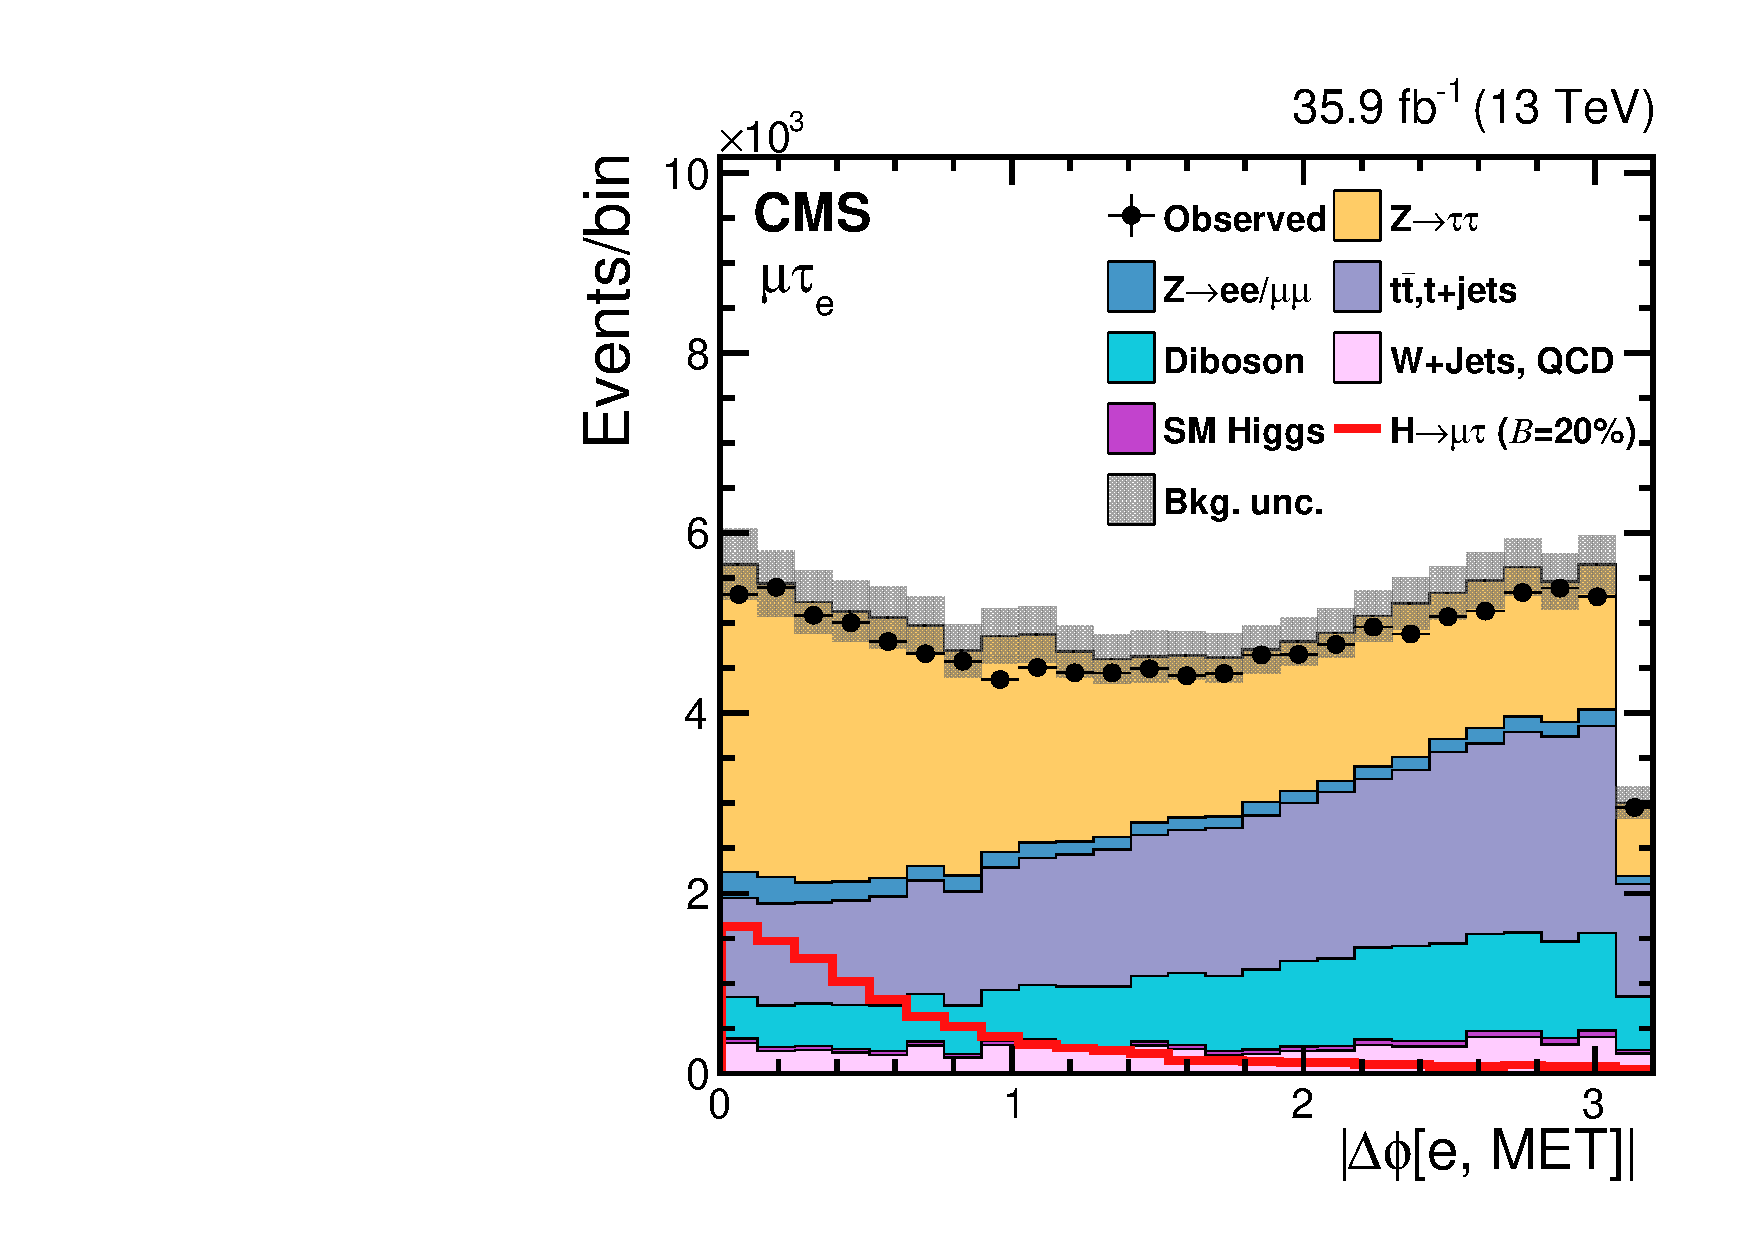
\includegraphics[width=0.315\textwidth]{plots_and_figures/chapter5/preselection/Figure_002-g.pdf}
 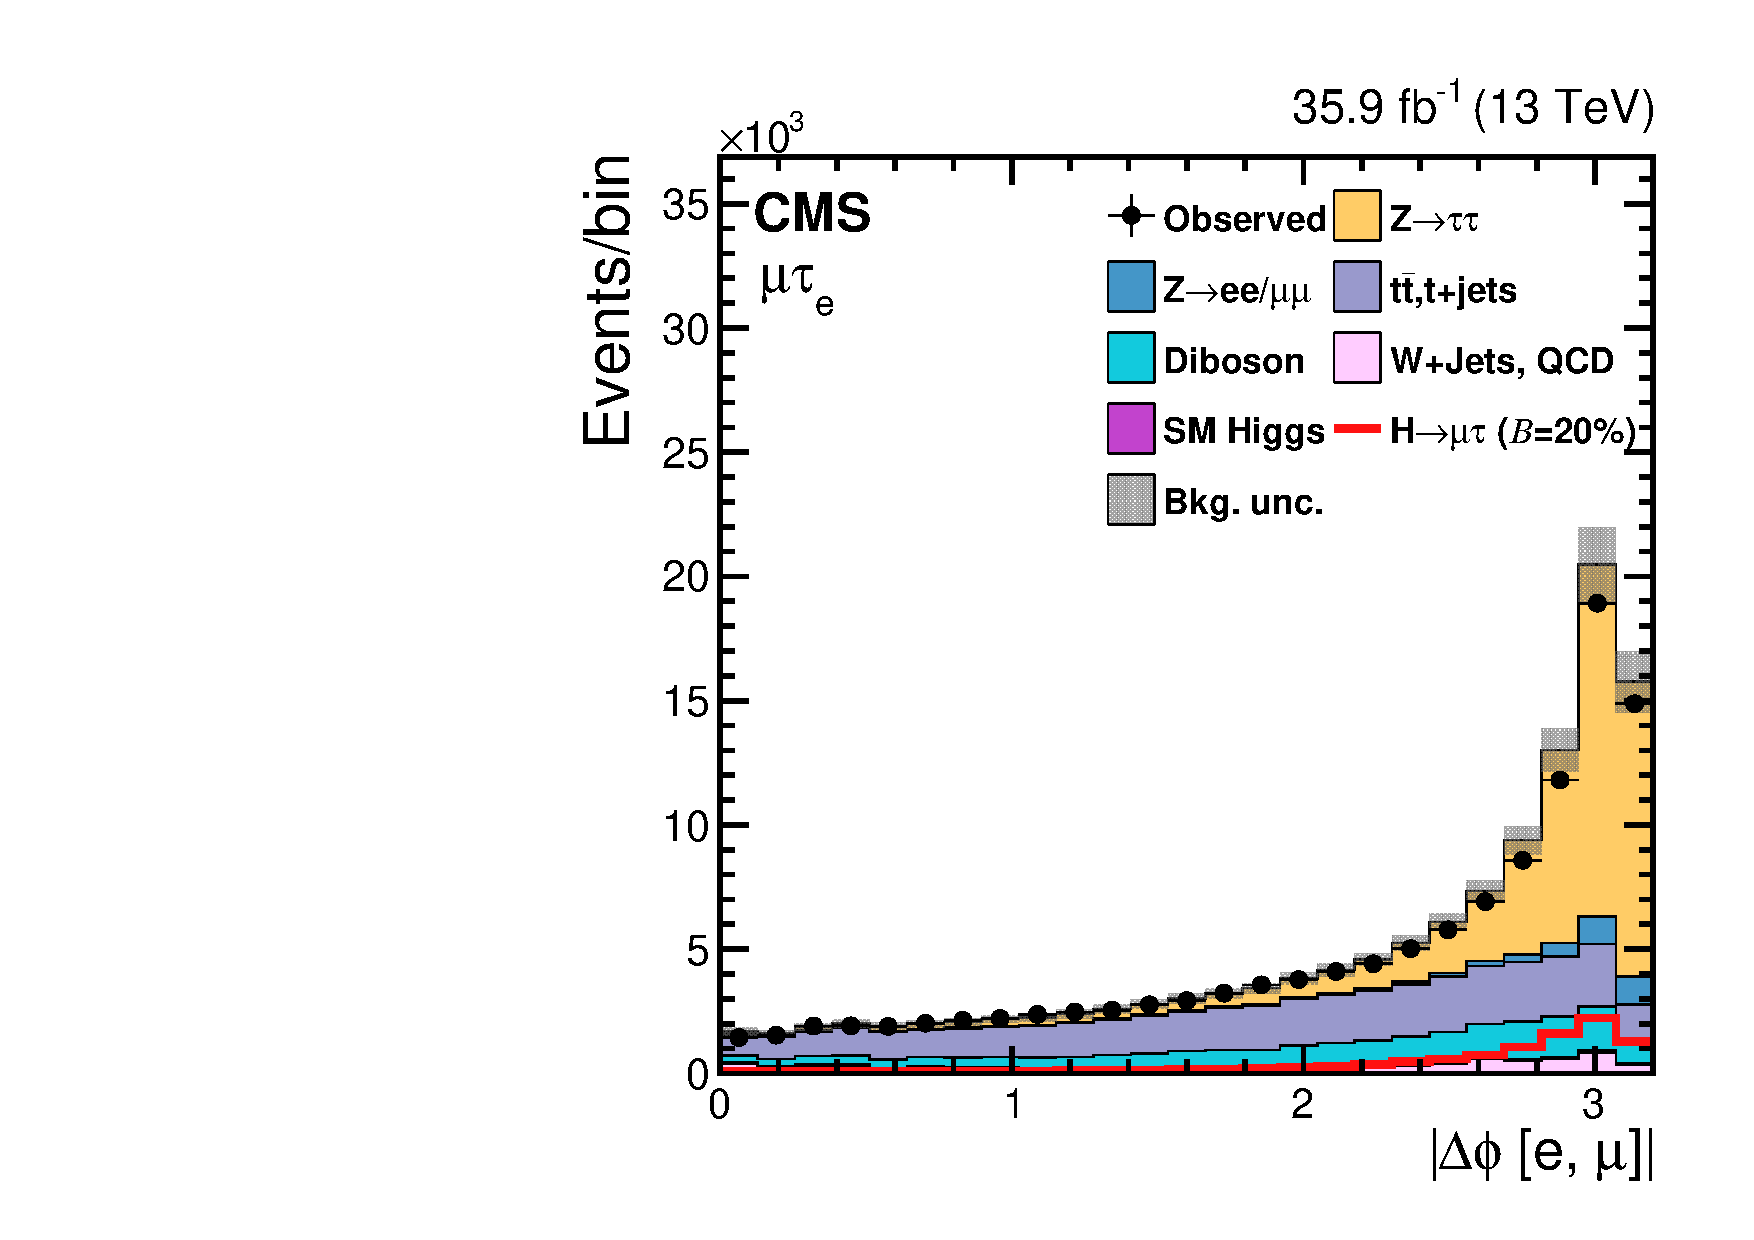
\includegraphics[width=0.315\textwidth]{plots_and_figures/chapter5/preselection/Figure_002-h.pdf}
\caption{Distributions of kinematic variables after baseline selction for \hmue analysis.}
 \label{fig:h125_presel}
\end{figure*}




\subsection{Cut Based Selection}
\label{h125_cb_sel}

\subsection{BDT Based Selection}
\label{h125_bdt_Sel}

\subsubsection{Boosted Decision Trees}
\label{bdts}


\section{Heavy Higgs Analysis}
\label{hh_evt_selec}

\subsection{Backgrounds}
\label{hh_evt_sel_bkg}









% % uncomment the following lines,
% if using chapter-wise bibliography
%
% \bibliographystyle{ndnatbib}
% \bibliography{example}
